% File: lecture_3.tex
\section{Advanced Entropy Coding \& Extensions}

\begin{center}
\textbf{Lecture 3: Beyond Huffman -- Advanced Entropy Coding Methods}
\end{center}

\subsection{Introduction \& Motivation}

\begin{importantbox}
\textbf{Recall Huffman Coding Limitations:}
\begin{itemize}
    \item \textbf{Integer code lengths}: Cannot reach entropy bound for highly skewed distributions
    \item \textbf{Static vs. Adaptive}: Standard Huffman requires prior knowledge of probabilities
    \item \textbf{Codebook overhead}: Need to transmit/store the coding tree
    \item \textbf{Symbol-by-symbol constraint}: Processes one symbol at a time
\end{itemize}
\end{importantbox}

\textbf{Lecture Roadmap:}
\begin{enumerate}
    \item \textbf{Framework}: Coding taxonomy and conceptual organization
    \item \textbf{Historical methods}: Shannon \& Shannon-Fano coding
    \item \textbf{Practical improvements}: Canonical and Adaptive Huffman
    \item \textbf{Next generation}: Arithmetic coding paradigm
    \item \textbf{Synthesis}: Comparison and forward look
\end{enumerate}

\subsection{Coding Taxonomy \& Framework}

\begin{definitionbox}
\textbf{Coding Taxonomy:} Classification of compression methods based on key characteristics
\end{definitionbox}

\begin{center}
\begin{tikzpicture}[node distance=1.5cm]
\node (compression) [rectangle, draw=black, thick, fill=blue!10, minimum width=3cm, minimum height=1cm] {\textbf{Compression Methods}};
\node (entropy) [below left=of compression, rectangle, draw=black, thick, fill=green!10, minimum width=2.5cm] {Entropy Coding};
\node (dictionary) [below right=of compression, rectangle, draw=black, thick, fill=orange!10, minimum width=2.5cm] {Dictionary Coding};
\node (shannon) [below=of entropy, rectangle, draw=black, fill=green!5, text width=2cm, align=center] {Shannon Coding};
\node (shannonfano) [below=of shannon, rectangle, draw=black, fill=green!5, text width=2cm, align=center] {Shannon-Fano};
\node (huffman) [below=of shannonfano, rectangle, draw=black, fill=green!5, text width=2cm, align=center] {Huffman};
\node (arithmetic) [below=of huffman, rectangle, draw=black, fill=green!5, text width=2cm, align=center] {Arithmetic};

\draw[->, thick] (compression) -- (entropy);
\draw[->, thick] (compression) -- (dictionary);
\draw[->] (entropy) -- (shannon);
\draw[->] (shannon) -- (shannonfano);
\draw[->] (shannonfano) -- (huffman);
\draw[->] (huffman) -- (arithmetic);
\end{tikzpicture}
\end{center}

\textbf{Key Dimensions in Compression Algorithm Design}

\begin{enumerate}
    \item \textbf{Modeling vs. Coding (Two-Stage View)}:
    \begin{itemize}
        \item \textbf{Modeling Phase}: Analyzes data to estimate symbol probabilities or discover patterns.
          \begin{itemize}
            \item \textit{Examples}: Frequency counting (Huffman), context modeling (PPM), dictionary construction (LZ77)
          \end{itemize}
        \item \textbf{Coding Phase}: Converts modeled information into actual bits.
          \begin{itemize}
            \item \textit{Examples}: Huffman codes, arithmetic codes, LZ77 pointers
          \end{itemize}
        \item Some algorithms intertwine both (e.g., LZW builds dictionary while coding).
    \end{itemize}
    
    \item \textbf{Knowledge of Source Distribution}:
    \begin{itemize}
        \item \textbf{Static/Fixed}: Uses a predefined model that doesn't change.
          \begin{itemize}
            \item \textit{Example}: JPEG Huffman tables, known language frequencies
            \item Requires prior knowledge of data; fails if distribution differs.
          \end{itemize}
        \item \textbf{Adaptive}: Learns and updates the model during compression.
          \begin{itemize}
            \item \textit{Example}: Adaptive Huffman, LZ78 dictionary building
            \item No prior knowledge needed; overhead for model transmission.
          \end{itemize}
        \item \textbf{Universal}: Can compress any source asymptotically optimally. 
          \begin{itemize}
            \item \textit{Theoretical property}: LZ family, arithmetic with adaptive model
            \item Note: Most adaptive methods are universal in practice.
          \end{itemize}
    \end{itemize}
    
    \item \textbf{Processing Granularity}:
    \begin{itemize}
        \item \textbf{Symbol-by-Symbol}: Each input symbol maps to one codeword.
          \begin{itemize}
            \item \textit{Example}: Huffman coding
            \item Simple but limited to integer bits per symbol.
          \end{itemize}
        \item \textbf{Block Coding}: Fixed-size groups of symbols coded together.
          \begin{itemize}
            \item \textit{Example}: Block-sorting (BWT) processes blocks
            \item Can capture inter-symbol dependencies within block.
          \end{itemize}
        \item \textbf{Stream/Incremental}: Continuous processing with immediate output.
          \begin{itemize}
            \item \textit{Example}: Arithmetic coding, LZ77 sliding window
            \item No blocking delay; good for real-time applications.
          \end{itemize}
        \item \textit{Note}: "Message-wide" (whole file as one symbol) is theoretical ideal; arithmetic coding approximates it by treating the entire stream as one long fractional code.
    \end{itemize}
    
    \item \textbf{Algorithmic Approach (Primary Taxonomy)}:
    \begin{itemize}
        \item \textbf{Statistical Coding}: Uses probability estimates (Huffman, Arithmetic)
        \item \textbf{Dictionary Coding}: Replaces repeated patterns with references (LZ family)
        \item \textbf{Transform Coding}: Changes data domain then codes (DCT, wavelet)
        \item \textbf{Predictive Coding}: Predicts next value, codes difference (DPCM, LPC)
    \end{itemize}
\end{enumerate}

\textbf{Important Relationships:}
\begin{itemize}
    \item Adaptive methods are usually universal for practical purposes.
    \item Stream coding is possible with both symbol-by-symbol (Huffman) and message-wide approaches (arithmetic).
    \item Block processing (like BWT) is often followed by stream coding (like MTF+RLE+arithmetic in bzip2).
    \item Modeling and coding can be separated (PPM + arithmetic) or combined (LZW).
\end{itemize}


\subsection{Shannon Coding (1948)}

\begin{definitionbox}
\textbf{Shannon Coding:} A constructive method derived from Shannon's source coding theorem that assigns codewords by taking the binary expansion of cumulative probabilities:
\[
l_i = \lceil -\log_2 p_i \rceil \quad \text{and} \quad \text{code}_i = \text{First } l_i \text{ bits of } F_i
\]
where \( p_i \) is the probability of symbol \( i \), and \( F_i = \sum_{j=1}^{i-1} p_j \) is the cumulative probability.
\end{definitionbox}

\begin{examplebox}
\textbf{Example:} Given symbols with probabilities:
\begin{center}
\begin{tabular}{c|c|c|c}
Symbol & Probability & $-\log_2 p_i$ & Cumulative $F_i$ \\
\hline
A & 0.5 & 1.0 & 0.0 \\
B & 0.25 & 2.0 & 0.5 \\
C & 0.125 & 3.0 & 0.75 \\
D & 0.125 & 3.0 & 0.875 \\
\end{tabular}
\end{center}

\textbf{Step-by-step construction:}
\begin{enumerate}
    \item \textbf{Calculate lengths:} $l_A = \lceil 1.0 \rceil = 1$, $l_B = 2$, $l_C = 3$, $l_D = 3$
    \item \textbf{Sort by probability} (already done above)
    \item \textbf{Compute cumulative probabilities:}
    \begin{itemize}
        \item $F_A = 0$ (first symbol)
        \item $F_B = 0.5$ (just A's probability)
        \item $F_C = 0.5 + 0.25 = 0.75$ (A + B)
        \item $F_D = 0.5 + 0.25 + 0.125 = 0.875$ (A + B + C)
    \end{itemize}
    \item \textbf{Convert $F_i$ to binary and take first $l_i$ bits:}
    \begin{itemize}
        \item \textbf{A:} $F_A = 0.0_{10}$ in binary is $0.0000\dots_2$
          \begin{itemize}
            \item Take first $l_A=1$ bit: $\mathbf{0}$
          \end{itemize}
        \item \textbf{B:} $F_B = 0.5_{10}$ in binary is $0.1000\dots_2$
          \begin{itemize}
            \item Take first $l_B=2$ bits: $\mathbf{10}$
          \end{itemize}
        \item \textbf{C:} $F_C = 0.75_{10}$ in binary is $0.1100\dots_2$
          \begin{itemize}
            \item Take first $l_C=3$ bits: $\mathbf{110}$
          \end{itemize}
        \item \textbf{D:} $F_D = 0.875_{10}$ in binary is $0.1110\dots_2$
          \begin{itemize}
            \item Take first $l_D=3$ bits: $\mathbf{111}$
          \end{itemize}
    \end{itemize}
\end{enumerate}

\textbf{Resulting code:}
\begin{center}
\begin{tabular}{c|c|c}
Symbol & Probability & Shannon Code \\
\hline
A & 0.5 & 0 \\
B & 0.25 & 10 \\
C & 0.125 & 110 \\
D & 0.125 & 111 \\
\end{tabular}
\end{center}

\textbf{Expected length:} $L = 0.5\times1 + 0.25\times2 + 0.125\times3 + 0.125\times3 = 1.75$ bits/symbol
\end{examplebox}

\begin{importantbox}
\textbf{Understanding the Binary Expansion Process:}

When we write $F_i$ in binary (e.g., $0.5 = 0.1_2$, $0.75 = 0.11_2$), we're essentially:
\begin{itemize}
    \item Dividing the interval [0,1) into subintervals based on probabilities
    \item Each symbol gets an interval of size $p_i$
    \item The codeword is the \textbf{binary fraction} representing the \textbf{start} of that interval
    \item We use exactly $l_i = \lceil -\log_2 p_i \rceil$ bits, which ensures:
    \[
    \frac{1}{2^{l_i}} \leq p_i < \frac{1}{2^{l_i-1}}
    \]
    \item This guarantees unique prefixes because intervals don't overlap!
\end{itemize}
\end{importantbox}

\begin{importantbox}
\textbf{Properties of Shannon Coding:}
\begin{itemize}
    \item \textbf{Constructive proof}: Demonstrates that prefix codes exist for any lengths satisfying Kraft inequality
    \item \textbf{Simple to compute}: Direct from probabilities, no tree needed
    \item \textbf{Not optimal}: Unlike Huffman, doesn't minimize expected length (compare: Huffman would give A=0, B=10, C=110, D=111 \textbf{same in this case!})
    \item \textbf{Theoretical importance}: Foundation for Shannon's source coding theorem
    \item \textbf{Efficiency bound}: $H(X) \leq L < H(X) + 1$ (like Shannon's theorem says)
\end{itemize}
\end{importantbox}


% here ....

% =========================================================
% Shannon–Fano Coding
% =========================================================
\subsection{Shannon–Fano Coding (1949)}

\begin{definitionbox}
\textbf{Shannon–Fano Coding:}
A top-down, recursive source coding technique that assigns binary codewords
by repeatedly partitioning a set of symbols into two subsets whose total
probabilities are as close as possible.  
The method was developed independently by \emph{Claude Shannon} and
\emph{Robert Fano} in 1949.
\end{definitionbox}

\subsubsection*{Algorithm Description}

\textbf{High-level idea:}  
Symbols with higher probabilities should receive shorter codewords.
This is achieved by repeatedly splitting the symbol set into two
probability-balanced groups and assigning binary prefixes.

\textbf{Step-by-step procedure:}
\begin{enumerate}
    \item \textbf{Sort} the symbols in decreasing order of probability:
    \[
    p_1 \ge p_2 \ge \cdots \ge p_n .
    \]

    \item \textbf{Recursive partitioning:}
    \begin{itemize}
        \item If the current set contains only one symbol, stop
        (this is the base case).
        \item Find an index $k$ that minimizes
        \[
        \Bigl|
        \sum_{i=1}^{k} p_i -
        \sum_{i=k+1}^{n} p_i
        \Bigr|.
        \]
        \item This divides the symbols into two subsets:
        \[
        S_1 = \{1,\ldots,k\}, \qquad
        S_2 = \{k+1,\ldots,n\}.
        \]
        \item Append bit \textbf{0} to the codewords of all symbols in $S_1$.
        \item Append bit \textbf{1} to the codewords of all symbols in $S_2$.
        \item Apply the same procedure recursively to $S_1$ and $S_2$.
    \end{itemize}
\end{enumerate}

% ---------------------------------------------------------
\subsubsection*{Example with Six Symbols}

\begin{examplebox}
\textbf{Example:} Consider six symbols with the following probabilities.

\begin{center}
\begin{tabular}{c|c|c}
Symbol & Probability & $-\log_2 p_i$ \\ \hline
A & 0.30 & 1.74 \\
B & 0.25 & 2.00 \\
C & 0.20 & 2.32 \\
D & 0.10 & 3.32 \\
E & 0.10 & 3.32 \\
F & 0.05 & 4.32
\end{tabular}
\end{center}

\textbf{Construction process}

\textbf{Step 1: First split} (balance $0.55$ vs.\ $0.45$)
\begin{itemize}
    \item Sorted symbols: A(0.30), B(0.25), C(0.20), D(0.10), E(0.10), F(0.05)
    \item Best split: $\{A,B\}(0.55)$ and $\{C,D,E,F\}(0.45)$
    \item Prefix assignment: $\{A,B\}\rightarrow 0$, $\{C,D,E,F\}\rightarrow 1$
\end{itemize}

\textbf{Step 2: Split $\{A,B\}$}
\begin{itemize}
    \item A: \textbf{00}, \quad B: \textbf{01}
\end{itemize}

\textbf{Step 3: Split $\{C,D,E,F\}$}
\begin{itemize}
    \item Best split: $\{C\}(0.20)$ and $\{D,E,F\}(0.25)$
    \item C: \textbf{10}, \quad $\{D,E,F\}\rightarrow 11$
\end{itemize}

\textbf{Step 4: Split $\{D,E,F\}$}
\begin{itemize}
    \item Best split: $\{D\}(0.10)$ and $\{E,F\}(0.15)$
    \item D: \textbf{110}, \quad $\{E,F\}\rightarrow 111$
\end{itemize}

\textbf{Step 5: Split $\{E,F\}$}
\begin{itemize}
    \item E: \textbf{1110}, \quad F: \textbf{1111}
\end{itemize}

\textbf{Final codes:}
\begin{center}
\begin{tabular}{c|c|c|c}
Symbol & Probability & Code & Length \\ \hline
A & 0.30 & 00   & 2 \\
B & 0.25 & 01   & 2 \\
C & 0.20 & 10   & 2 \\
D & 0.10 & 110  & 3 \\
E & 0.10 & 1110 & 4 \\
F & 0.05 & 1111 & 4
\end{tabular}
\end{center}

\textbf{Expected code length:}
\[
L = 2.40 \text{ bits/symbol}.
\]

\textbf{Entropy:}
\[
H(X) \approx 2.25 \text{ bits/symbol}.
\]

\textbf{Efficiency:}
\[
\frac{H(X)}{L} \approx 93.8\%.
\]
\end{examplebox}

% ---------------------------------------------------------
\subsubsection*{Visual Tree Representation}

\begin{center}
\scriptsize
\begin{verbatim}
                                    ROOT
                                   /    \
                                 0/      \1
                                 /        \
                          {A,B} 0.55    {C,D,E,F} 0.45
                             / \            / \
                           0/   \1        0/   \1
                           /     \         /     \
                   {A} 0.30  {B} 0.25  {C} 0.20  {D,E,F} 0.25
                     00        01        10         / \
                                                  0/   \1
                                                  /     \
                                            {D} 0.10  {E,F} 0.15
                                              110        / \
                                                       0/   \1
                                                       /     \
                                                 {E} 0.10  {F} 0.05
                                                   1110      1111
\end{verbatim}
\end{center}

\subsubsection*{Key Observations}

\begin{itemize}
    \item \textbf{Probability-balanced splits:} The algorithm focuses on
    balancing probabilities rather than the number of symbols.
    \item \textbf{Variable code lengths:} More probable symbols receive
    shorter codewords.
    \item \textbf{Prefix-free property:} No codeword is a prefix of another.
    \item \textbf{Near-optimal performance:} The efficiency is high but not
    guaranteed to be optimal.
\end{itemize}

\begin{importantbox}
\textbf{Limitations and Historical Context}
\begin{itemize}
    \item Shannon–Fano coding does \emph{not} always produce the optimal code.
    \item Huffman coding (1952) guarantees the minimum average code length.
    \item Historically important as a precursor to Huffman coding.
\end{itemize}
\end{importantbox}


%-------------------------------------------------
\subsection{Canonical Huffman Codes}
%-------------------------------------------------

\begin{definitionbox}
\textbf{Canonical Huffman Code:}
A standardized representation of a Huffman code in which:
\begin{itemize}
    \item Codes are assigned in lexicographic (binary) order
    \item All codewords of the same length are consecutive binary numbers
    \item The first codeword of each length is the smallest possible binary value
\end{itemize}
Only the code lengths are required to reconstruct the entire code.
This enables compact storage and fast table-based decoding.
\end{definitionbox}

\subsubsection*{Why Canonical Huffman Codes?}

A standard Huffman algorithm produces \emph{optimal code lengths}, but the exact
bit patterns depend on implementation details such as tie-breaking and tree
construction:
\begin{itemize}
    \item Different trees can yield the same optimal set of code lengths
    \item Different bit assignments, but identical compression performance
\end{itemize}

Canonical Huffman coding fixes \textbf{one unique and deterministic assignment}
for a given set of code lengths so that:
\begin{enumerate}
    \item Only code lengths need to be transmitted
    \item The decoder can reconstruct the codes without ambiguity
    \item Decoding can be implemented efficiently using lookup tables
\end{enumerate}

\subsubsection*{Two-Step Process}

\textbf{Complete workflow:}
\begin{enumerate}
    \item \textbf{Run the standard Huffman algorithm} to obtain optimal code lengths $l_i$
    \item \textbf{Apply the canonical transformation} to convert lengths into standardized codes
\end{enumerate}

\begin{center}
\fbox{
\begin{minipage}{0.8\textwidth}
\centering
Symbol probabilities
$\;\xrightarrow{\text{Huffman}}\;$
Code lengths
$\;\xrightarrow{\text{Canonical}}\;$
Canonical codes
\end{minipage}
}
\end{center}

\subsubsection*{Canonical Code Construction Algorithm}

\textbf{Input:} Code lengths $l_i$ obtained from a standard Huffman algorithm  
\textbf{Output:} Canonical Huffman codes

\begin{algorithm}[H]
\caption{Canonical Huffman Construction}
\begin{algorithmic}[1]
\Require Code lengths $l_1, \dots, l_n$
\Ensure Canonical codes $c_1, \dots, c_n$
\State Sort symbols by $(l_i, \text{symbol index})$
\State $l_{\min} \gets \min\{l_i\}$, $l_{\max} \gets \max\{l_i\}$
\For{$l = l_{\min}$ to $l_{\max}$}
    \State $count[l] \gets 0$ \Comment{Initialize count array}
\EndFor
\For{each symbol $i$}
    \State $count[l_i] \gets count[l_i] + 1$ \Comment{Count symbols per length}
\EndFor
\State $next[l_{\min}] \gets 0$
\For{$l = l_{\min}+1$ to $l_{\max}$}
    \State $next[l] \gets (next[l-1] + count[l-1]) \times 2$
\EndFor
\For{each symbol $i$ (in sorted order) with length $l_i$}
    \State $c_i \gets$ binary($next[l_i]$, $l_i$) \Comment{Convert to $l_i$-bit binary}
    \State $next[l_i] \gets next[l_i] + 1$
\EndFor
\end{algorithmic}
\end{algorithm}

\textbf{Detailed step-by-step explanation:}

\begin{enumerate}
    \item \textbf{Sort symbols:}
    \begin{enumerate}
        \item Primary key: increasing code length $l_i$
        \item Secondary key: symbol value (or symbol index)
    \end{enumerate}

    \item \textbf{Count symbols per length:}  
    Let $L_{\min}$ and $L_{\max}$ be the minimum and maximum code lengths.
    For each length $l$, compute:
    \[
    \text{count}[l] = \text{number of symbols with length } l
    \]

    \item \textbf{Compute starting codes:}  
    Initialize the first starting code:
    \[
    \text{start\_code}[L_{\min}] = 0
    \]
    For each length $l = L_{\min}+1$ to $L_{\max}$:
    \[
    \text{start\_code}[l]
    =
    \bigl(\text{start\_code}[l-1] + \text{count}[l-1]\bigr)\times 2
    \]

    \item \textbf{Initialize assignment pointers:}
    \[
    \text{next\_code}[l] = \text{start\_code}[l]
    \quad \text{for all } l
    \]

    \item \textbf{Assign codes to symbols:}
    \begin{itemize}
        \item Traverse the sorted symbol list
        \item For each symbol of length $l$:
        \begin{itemize}
            \item Assign the current value of $\text{next\_code}[l]$
            \item Increment $\text{next\_code}[l]$ by one
        \end{itemize}
    \end{itemize}
\end{enumerate}

\subsubsection*{Understanding the Shift Operation}

\textbf{Key idea:}  
All codes of length $l+1$ must begin immediately after the last code of length $l$,
and must be exactly one bit longer.

If the last code of length $l$ has integer value $x$, then the first code of length
$l+1$ is:
\[
\text{start\_code}[l+1] = (x + 1)\times 2
\]

In binary representation, this corresponds to:
\[
(x+1)_2 \text{ followed by a } 0
\]

This construction ensures:
\begin{itemize}
    \item Prefix-free property
    \item Lexicographic ordering is preserved
    \item No overlap between different length groups
\end{itemize}

\subsubsection*{Complete Worked Example}

\begin{examplebox}
\textbf{Example:} Suppose the Huffman algorithm produces the following code lengths:

\begin{center}
\begin{tabular}{c|c}
Symbol & Length $(l_i)$ \\ \hline
A & 2 \\
B & 3 \\
C & 3 \\
D & 3 \\
E & 4 \\
F & 4
\end{tabular}
\end{center}

\textbf{Step 1: Sort symbols by length, then by symbol order}
\begin{itemize}
    \item Length 2: A
    \item Length 3: B, C, D
    \item Length 4: E, F
\end{itemize}

\textbf{Step 2: Count symbols per length}
\[
\text{count}[2]=1,\qquad
\text{count}[3]=3,\qquad
\text{count}[4]=2
\]

\textbf{Step 3: Compute starting codes}
\begin{align*}
\text{start\_code}[2] &= 0 \quad (00_2) \\
\text{start\_code}[3] &= (0 + 1)\times 2 = 2 \quad (010_2) \\
\text{start\_code}[4] &= (2 + 3)\times 2 = 10 \quad (1010_2)
\end{align*}

\textbf{Step 4: Initialize assignment pointers}
\[
\text{next\_code}[2]=0,\quad
\text{next\_code}[3]=2,\quad
\text{next\_code}[4]=10
\]

\textbf{Step 5: Assign codes}
\begin{center}
\begin{tabular}{c|c|l|c|c}
Symbol & Length & Action & Code & $\text{next\_code}[l]$ after \\ \hline
A & 2 & Assign $\text{next\_code}[2]=0$ & 00 & 1 \\
B & 3 & Assign $\text{next\_code}[3]=2$ & 010 & 3 \\
C & 3 & Assign $\text{next\_code}[3]=3$ & 011 & 4 \\
D & 3 & Assign $\text{next\_code}[3]=4$ & 100 & 5 \\
E & 4 & Assign $\text{next\_code}[4]=10$ & 1010 & 11 \\
F & 4 & Assign $\text{next\_code}[4]=11$ & 1011 & 12
\end{tabular}
\end{center}

\textbf{Final canonical codes:}
\begin{center}
\begin{tabular}{c|c|c}
Symbol & Length & Canonical Code \\ \hline
A & 2 & 00 \\
B & 3 & 010 \\
C & 3 & 011 \\
D & 3 & 100 \\
E & 4 & 1010 \\
F & 4 & 1011
\end{tabular}
\end{center}
\end{examplebox}

\subsubsection*{Transmission and Decoding}

\textbf{Transmission format:}
\begin{itemize}
    \item Transmit only the sequence of code lengths:
    \[
    \langle l_1, l_2, \dots, l_n \rangle
    \]
    \item Example: $\langle 2, 3, 3, 3, 4, 4 \rangle$
    \item Each length can be represented using
    $\lceil \log_2 L_{\max} \rceil$ bits
\end{itemize}

\textbf{Decoder operation:}
\begin{enumerate}
    \item Read code lengths for all symbols
    \item Reconstruct canonical codes using the same algorithm
    \item Build a decoding table mapping $(\text{code}, \text{length})$ to symbols
    \item Decode the bitstream using table lookup
\end{enumerate}

\subsubsection*{Comparison with Standard Huffman}

\begin{center}
\renewcommand{\arraystretch}{1.2}
\begin{tabular}{|p{6cm}|p{6cm}|}
\hline
\textbf{Standard Huffman (tree-based)} & \textbf{Canonical Huffman (length-based)} \\ \hline
Output: Huffman tree & Output: Code lengths \\ \hline
Must transmit tree structure & Transmit only lengths \\ \hline
Decoding by tree traversal & Decoding by table lookup \\ \hline
Multiple equivalent trees & Single deterministic assignment \\ \hline
Same optimal compression & Same optimal compression \\ \hline
More complex implementation & Simple, robust implementation \\ \hline
\end{tabular}
\end{center}

\subsubsection*{Key Properties}

\begin{itemize}
    \item \textbf{Optimality:} Identical compression ratio to standard Huffman
    \item \textbf{Compactness:} Only code lengths are stored or transmitted
    \item \textbf{Speed:} Table-based decoding is significantly faster
    \item \textbf{Standardization:} Used in DEFLATE (gzip/ZIP), JPEG, PNG, MPEG
\end{itemize}

\begin{importantbox}
\textbf{Critical Insight:}
Canonical Huffman coding is \textbf{not} a different compression algorithm.
The Huffman algorithm determines \emph{how long} each code should be,
while the canonical transformation determines the \emph{exact bit patterns}
in a consistent and reproducible manner.
\end{importantbox}


\subsection{Adaptive Huffman Coding}

\subsubsection{Overview}

\begin{definitionbox}
\textbf{Adaptive Huffman Coding} is a single-pass, lossless data compression
technique in which the Huffman model is updated dynamically as symbols are
encoded and decoded. The Huffman tree evolves on-the-fly, allowing both the
encoder and decoder to adapt to changing symbol statistics without any prior
knowledge of the source distribution.
\end{definitionbox}

Unlike static Huffman coding, adaptive Huffman coding does not require a
preprocessing phase to compute symbol frequencies. Instead, symbol statistics
are learned incrementally as the data stream is processed.


\subsubsection{Limitations of Static Huffman Coding}

Static Huffman coding assumes that symbol statistics are known in advance:
\begin{itemize}
    \item Requires two passes over the data:
    \begin{enumerate}
        \item Collect symbol frequencies
        \item Encode using the constructed Huffman tree
    \end{enumerate}
    \item The Huffman tree (or code lengths) must be transmitted as side
    information
    \item Cannot adapt to non-stationary or evolving symbol distributions
\end{itemize}

These limitations motivate adaptive schemes when symbol statistics are unknown
or change over time.


\subsubsection{Key Principle of Adaptive Huffman Coding}

Adaptive Huffman coding maintains a Huffman tree that is updated after encoding
or decoding each symbol.

\textbf{Key invariant:} After processing each symbol, the encoder and decoder
maintain \emph{identical Huffman trees} by applying the same updates in the same
order. This ensures correct decoding without transmitting the tree explicitly.


\subsubsection{Initialization}

The algorithm begins with a special symbol:
\begin{itemize}
    \item A single \textbf{NYT} (Not Yet Transmitted) node
\end{itemize}

When a symbol appears for the first time:
\begin{itemize}
    \item The code for the NYT node is output
    \item The raw symbol value is transmitted
    \item The NYT node is expanded into:
    \begin{itemize}
        \item A new NYT node
        \item A leaf node representing the new symbol
    \end{itemize}
\end{itemize}

\emph{Note: Some variants preinitialize the tree if the alphabet is fixed, but
the standard adaptive Huffman algorithm begins with only the NYT node.}


\subsubsection{Tree Update Mechanism}

After each symbol is processed:
\begin{itemize}
    \item The frequency (weight) of the corresponding leaf node is incremented
    \item The tree is updated to preserve the \textbf{sibling property}
\end{itemize}

\begin{definitionbox}
\textbf{Sibling Property:}
Nodes are numbered such that nodes with higher weights have higher numbers.
For any given weight, all nodes with that weight form a contiguous block.
Each internal node has exactly two children.
\end{definitionbox}

To restore this property, nodes may be swapped with others of equal weight,
followed by incrementing parent node weights. This update process proceeds
bottom-up toward the root.


\subsubsection{Encoding and Decoding Process}

\begin{itemize}
    \item If the symbol has appeared before:
    \begin{itemize}
        \item Output its current Huffman code
    \end{itemize}
    \item If the symbol is new:
    \begin{itemize}
        \item Output the code for the NYT node
        \item Output the symbol in raw (fixed-length) form
    \end{itemize}
    \item Update the tree identically at both encoder and decoder
\end{itemize}

\emph{Note: Exact bit patterns depend on the update order and implementation.
Adaptive Huffman coding guarantees prefix-free optimality but not unique codes.}


\subsubsection{Algorithms}

Two classical adaptive Huffman algorithms are widely used:
\begin{itemize}
    \item \textbf{FGK Algorithm} (Faller--Gallager--Knuth)
    \item \textbf{Vitter's Algorithm (Algorithm V)}, which improves worst-case
    performance and is commonly preferred
\end{itemize}

Both algorithms maintain the sibling property while ensuring efficient updates.


\subsubsection{Performance Characteristics}

\begin{itemize}
    \item Update cost is \textbf{amortized} $O(1)$ per symbol
    \item Worst-case update time is proportional to the tree height
    \item Compression efficiency:
    \begin{itemize}
        \item Initially suboptimal
        \item Converges toward entropy-optimal coding as statistics stabilize
    \end{itemize}
\end{itemize}


\subsubsection{Comparison with Static Huffman Coding}

\begin{center}
\begin{tabular}{lcc}
\toprule
\textbf{Feature} & \textbf{Static Huffman} & \textbf{Adaptive Huffman} \\
\midrule
Number of passes & Two & One \\
Prior statistics required & Yes & No \\
Model transmission & Required & Not required \\
Adaptation to changes & No & Yes \\
Initial efficiency & High & Low \\
Asymptotic efficiency & Optimal & Near-optimal \\
\bottomrule
\end{tabular}
\end{center}


\subsubsection{Applications}

Adaptive Huffman coding is well suited for:
\begin{itemize}
    \item Streaming data sources
    \item Real-time communication
    \item Situations where full statistics cannot be collected in advance
\end{itemize}

However, it may be less suitable when symbol distributions are known and stable,
or when computational simplicity is critical.


\subsubsection{Summary}

Adaptive Huffman coding extends classical Huffman coding to dynamic environments.
By updating the coding model incrementally and maintaining strict structural
invariants, it enables efficient, single-pass compression without prior
knowledge of source statistics.



\subsection{Arithmetic Coding: The Paradigm Shift}

\begin{definitionbox}
\textbf{Arithmetic Coding:} Encodes an entire message into a single fractional number in the interval $[0,1)$, approaching the entropy bound very closely.
\end{definitionbox}

\textbf{Core Idea:} Represent messages as subintervals of $[0,1)$:

\begin{center}
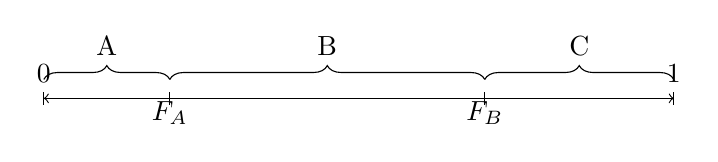
\begin{tikzpicture}[scale=0.8]
\draw[<->] (0,0) -- (10,0);
\draw (0,-0.1) -- (0,0.1) node[above] {0};
\draw (10,-0.1) -- (10,0.1) node[above] {1};
\draw (2,-0.1) -- (2,0.1) node[below] {$F_{A}$};
\draw (7,-0.1) -- (7,0.1) node[below] {$F_{B}$};
\draw[decorate,decoration={brace,amplitude=5pt}] (0,0.3) -- (2,0.3) node[midway,above=5pt] {A};
\draw[decorate,decoration={brace,amplitude=5pt}] (2,0.3) -- (7,0.3) node[midway,above=5pt] {B};
\draw[decorate,decoration={brace,amplitude=5pt}] (7,0.3) -- (10,0.3) node[midway,above=5pt] {C};
\end{tikzpicture}
\end{center}

\begin{algorithm}
\caption{Arithmetic Encoding Algorithm}
\begin{algorithmic}[1]
\Require Message $m = s_1 s_2 \dots s_k$, symbol probabilities $p_i$
\Ensure Final interval $[low, high)$
\State $low \gets 0.0$, $high \gets 1.0$
\For{each symbol $s$ in $m$}
    \State $range \gets high - low$
    \State $high \gets low + range \times F_s$ \Comment{$F_s$: cumulative prob up to $s$}
    \State $low \gets low + range \times F_{s-1}$ \Comment{$F_{s-1}$: cumulative prob before $s$}
\EndFor
\Return any number in $[low, high)$
\end{algorithmic}
\end{algorithm}

\begin{examplebox}
\textbf{Example:} Encode message "CAB" with probabilities: A(0.5), B(0.25), C(0.25)

\begin{center}
\begin{tabular}{c|c|c}
Symbol & Probability & Cumulative \\
\hline
A & 0.5 & 0.5 \\
B & 0.25 & 0.75 \\
C & 0.25 & 1.0 \\
\end{tabular}
\end{center}

\textbf{Encoding:}
\begin{enumerate}
    \item Start: $[0, 1)$
    \item Process 'C': $[0.75, 1.0)$ \quad (C occupies $[0.75, 1.0)$)
    \item Process 'A': $range = 0.25$
        \begin{itemize}
            \item $low = 0.75 + 0.25 \times 0.0 = 0.75$
            \item $high = 0.75 + 0.25 \times 0.5 = 0.875$
            \item New interval: $[0.75, 0.875)$
        \end{itemize}
    \item Process 'B': $range = 0.125$
        \begin{itemize}
            \item $low = 0.75 + 0.125 \times 0.5 = 0.8125$
            \item $high = 0.75 + 0.125 \times 0.75 = 0.84375$
            \item Final interval: $[0.8125, 0.84375)$
        \end{itemize}
\end{enumerate}
\textbf{Output:} Any number in $[0.8125, 0.84375)$, e.g., 0.8125 in binary
\end{examplebox}

\begin{importantbox}
\textbf{Practical Implementation Issues:}
\begin{itemize}
    \item \textbf{Finite precision}: Use integer arithmetic with scaling
    \item \textbf{Renormalization}: Output bits when interval confined to one half
    \item \textbf{Carry-over}: Handle when interval spans midpoint
    \item \textbf{Termination}: Need special end-of-message symbol
\end{itemize}
\end{importantbox}

\textbf{Adaptive Arithmetic Coding:} Easier than adaptive Huffman - just update probabilities as you go!

\subsection{Comparison \& Synthesis}

% Fixed table to fit within margins
\begin{center}
\small % Use smaller font for table
\begin{tabular}{|p{2.5cm}|c|c|c|c|p{2.5cm}|}
\hline
\textbf{Method} & \textbf{Optimal?} & \textbf{Adaptive?} & \textbf{Complexity} & \textbf{Near Entropy?} & \textbf{Key Applications} \\
\hline
Shannon Coding & No & No & Low & No & Theoretical proofs \\
\hline
Shannon-Fano & No & No & Low & Sometimes & Historical \\
\hline
Huffman & Yes* & No & Low & Moderate & General purpose \\
\hline
Canonical Huffman & Yes* & No & Low & Moderate & DEFLATE, JPEG, PNG \\
\hline
Adaptive Huffman & Yes* & Yes & Medium & Moderate & Early compressors \\
\hline
Arithmetic Coding & \textbf{Near-opt} & \textbf{Yes} & \textbf{High} & \textbf{Yes (close)} & \textbf{JPEG2000, H.264, HEVC} \\
\hline
\end{tabular}
\end{center}
\smallskip
*Optimal for symbol-by-symbol coding given probabilities

\begin{importantbox}
\textbf{Key Insights:}
\begin{itemize}
    \item \textbf{Huffman vs. Arithmetic}: Huffman is simpler but has an "integer penalty"; Arithmetic approaches entropy bound
    \item \textbf{Modern standards}: Arithmetic coding (CABAC) used in video compression for 10-20\% better compression
    \item \textbf{Practical choice}: For general compression, Canonical Huffman (DEFLATE); for media, Arithmetic coding
    \item \textbf{The missing piece}: All these methods assume we have good probability estimates. Where do those come from?
\end{itemize}
\end{importantbox}

\subsection{Forward Look}

\textbf{The Complete Picture: What Comes Next?}

\begin{center}
\begin{tikzpicture}[node distance=1.8cm]
\node (lecture1) [rectangle, draw=black, thick, fill=blue!10, minimum width=3cm, minimum height=1cm] {\parbox{2.8cm}{\centering \textbf{Lecture 1}\\Huffman Coding}};
\node (lecture2) [below=of lecture1, rectangle, draw=black, thick, fill=green!10, minimum width=3cm, minimum height=1cm] {\parbox{2.8cm}{\centering \textbf{Lecture 2}\\Theory\\Entropy, Kraft-McMillan}};
\node (lecture3) [below=of lecture2, rectangle, draw=black, thick, fill=orange!10, minimum width=3cm, minimum height=1cm] {\parbox{2.8cm}{\centering \textbf{Lecture 3}\\Advanced Coding\\Arithmetic, Canonical}};
\node (lecture4) [below=of lecture3, rectangle, draw=black, thick, fill=red!10, minimum width=3cm, minimum height=1cm] {\parbox{2.8cm}{\centering \textbf{Lecture 4}\\Source Modeling\\Markov, Context}};
\node (lecture5) [below=of lecture4, rectangle, draw=black, thick, fill=purple!10, minimum width=3cm, minimum height=1cm] {\parbox{2.8cm}{\centering \textbf{Lecture 5}\\Dictionary Methods\\LZ Family}};

\draw[->, thick] (lecture1) -- (lecture2);
\draw[->, thick] (lecture2) -- (lecture3);
\draw[->, thick] (lecture3) -- (lecture4);
\draw[->, thick] (lecture4) -- (lecture5);
\end{tikzpicture}
\end{center}

\textbf{Next Lecture: Source Modeling and Statistical Dependence}
\begin{itemize}
    \item \textbf{The missing half}: We now know how to code efficiently, but where do the probabilities come from?
    \item \textbf{Real data has memory}: 'Q' is usually followed by 'U' in English text
    \item \textbf{Markov models}: Capturing dependencies between symbols
    \item \textbf{Context modeling}: Using past symbols to predict future ones
    \item \textbf{The modeling-coding separation}: Modern compressors separate these two tasks
\end{itemize}

\textbf{The Big Question for Next Time:}
\begin{center}
\fbox{\parbox{0.8\textwidth}{\centering
\textbf{If Arithmetic coding can get within 0.01 bits of entropy,\\ 
what's the real limit to compression?\\ 
The answer: It's not the coding, it's the \textit{modeling}!}}
}
\end{center}

\textbf{The Two Pillars of Compression (Revised View):}
\begin{center}
\begin{tikzpicture}[node distance=2cm]
\node (comp) [rectangle, draw=black, thick, minimum width=8cm, minimum height=2cm] {\textbf{Data Compression}};
\node (modeling) [below left=1cm of comp.south, rectangle, draw=red, thick, fill=red!5, minimum width=3.5cm, minimum height=1.2cm] {\parbox{3.2cm}{\centering \textbf{Modeling}\\Probability Estimation\\90\% of compression gain}};
\node (coding) [below=of comp, rectangle, draw=blue, thick, fill=blue!5, minimum width=3.5cm, minimum height=1.2cm] {\parbox{3.2cm}{\centering \textbf{Coding}\\Bit Assignment\\10\% of compression gain}};
\node (dictionary) [below right=1cm of comp.south, rectangle, draw=green, thick, fill=green!5, minimum width=3.5cm, minimum height=1.2cm] {\parbox{3.2cm}{\centering \textbf{Dictionary}\\Repetition-based\\Different approach}};

\draw[->, thick, red] (comp.south) -- (modeling);
\draw[->, thick, blue] (comp.south) -- (coding);
\draw[->, thick, green] (comp.south) -- (dictionary);

\node (modeltech) [below=0.5cm of modeling] {\parbox{3.2cm}{\centering Markov Models\\Context Modeling\\PPM}};
\node (codetech) [below=0.5cm of coding] {\parbox{3.2cm}{\centering Huffman\\Arithmetic\\Canonical}};
\node (dicttech) [below=0.5cm of dictionary] {\parbox{3.2cm}{\centering LZ77, LZ78\\LZW\\DEFLATE}};

\draw[red!50] (modeling) -- (modeltech);
\draw[blue!50] (coding) -- (codetech);
\draw[green!50] (dictionary) -- (dicttech);
\end{tikzpicture}
\end{center}

\begin{exercisebox}
\textbf{Exercise 3.1:} Given symbols with probabilities: A(0.4), B(0.3), C(0.2), D(0.1)
\begin{enumerate}[label=(\alph*)]
    \item Construct a Shannon code and compute its expected length
    \item Construct a Shannon-Fano code
    \item Compare with Huffman code from Lecture 2
\end{enumerate}
\end{exercisebox}

\begin{exercisebox}
\textbf{Exercise 3.2:} Convert the following Huffman code to canonical form:
\begin{center}
\begin{tabular}{c|c}
Symbol & Huffman Code \\
\hline
A & 0 \\
B & 100 \\
C & 101 \\
D & 110 \\
E & 1110 \\
F & 1111 \\
\end{tabular}
\end{center}
\end{exercisebox}

\begin{exercisebox}
\textbf{Exercise 3.3:} Encode the message "ABAC" using arithmetic coding with probabilities: A(0.6), B(0.3), C(0.1). Show each step.
\end{exercisebox}

\begin{exercisebox}
\textbf{Exercise 3.4: Thinking Ahead:} Consider the English phrase "THE QUICK BROWN FOX"
\begin{enumerate}[label=(\alph*)]
    \item If we use Huffman coding with letter frequencies, what's wrong with this approach?
    \item How might knowing that 'Q' is usually followed by 'U' help compression?
    \item Why would arithmetic coding be better than Huffman for this kind of data?
\end{enumerate}
\end{exercisebox}

\vspace{1cm}
\begin{center}
\rule{0.8\textwidth}{0.5pt}\\
\textbf{End of Lecture 3 -- Advanced Entropy Coding Methods}\\
\textbf{Next: Lecture 4 -- Source Modeling and Statistical Dependence}\\
\textit{We now have efficient coding methods. Next: Where do the probabilities come from?}
\end{center}
